\documentclass{beamer}
\usepackage{graphicx, amsmath}

\title{GRSC 7770 Graduate Seminar}
\subtitle{A field guide to teaching MATH 1113}
\author{William E. Olsen}
\date{\today}

\begin{document}
\frame{\titlepage}

\begin{frame}
  \begin{block}{Question}
    Does it even matter if I do a good job of teaching MATH 1113?
  \end{block}
\end{frame}

\begin{frame}
  \begin{block}{Albert Einstein}
    ``It's a miracle that curiosity survives formal education.''
  \end{block}
  
\end{frame}

\begin{frame}
  \frametitle{STEM Entrance}
  \begin{itemize}
  \item  About 28\% of 2003-04 beginning bachelor degree students choose a STEM major at some point during their enrollment between 2003 and 2009 (see Figure 1).
  \item Within STEM fields, biological/life sciences was the most popular field, attracting 11\% of bachelor's degree students.
  \item Mathematics and physical sciences were the two least popular fields, with $\sim 3\%$ of students. 
  \end{itemize}
\end{frame}

\begin{frame}
  \frametitle{STEM Entrance}
  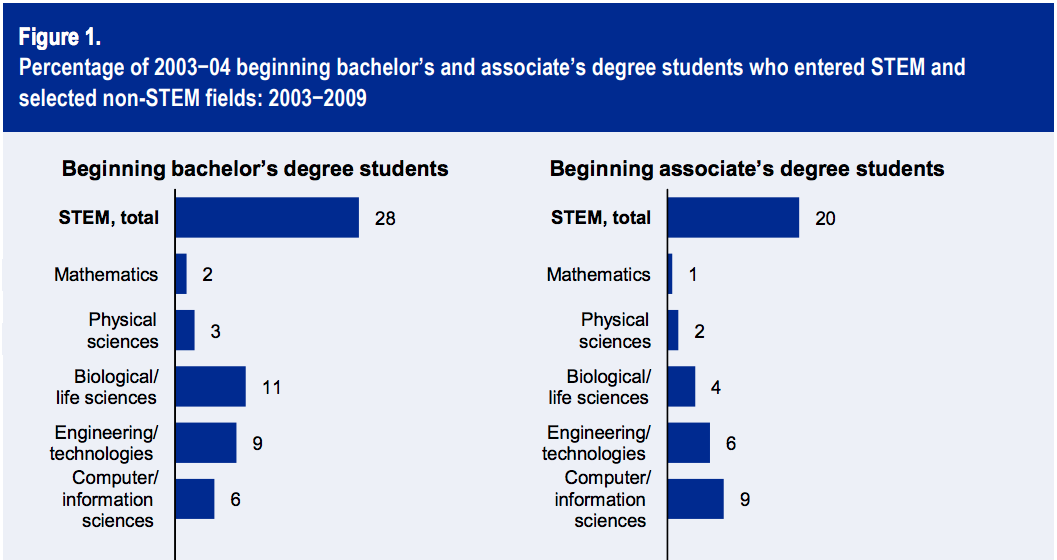
\includegraphics[scale = 0.34]{fig1.png}
\end{frame}

\begin{frame}
  \frametitle{STEM Attrition}
  \begin{block}{Question}
    Ok. STEM starts out small, but we keep everyone who comes in, right?
  \end{block}
\end{frame}

\begin{frame}
  \frametitle{STEM Attrition}
  \centering
  \textsc{nope}.
\end{frame}

\begin{frame}
  \frametitle{STEM Attrition}
  \begin{itemize}
  \item Among bachelor's degree students entering STEM fields between 2003 and 2009, nearly one-half (48\%) had left these fields by spring 2009 (fig. 2).
  \item Some left STEM by switching their major (28\%).
  \item Some left STEM by dropping out of university all together (20\%).
  \item Attrition rates varied across STEM disciplines-- 38\% for mathematics and 59\% for computer/information science majors.
  \end{itemize} 
\end{frame}

\begin{frame}
  \centering
  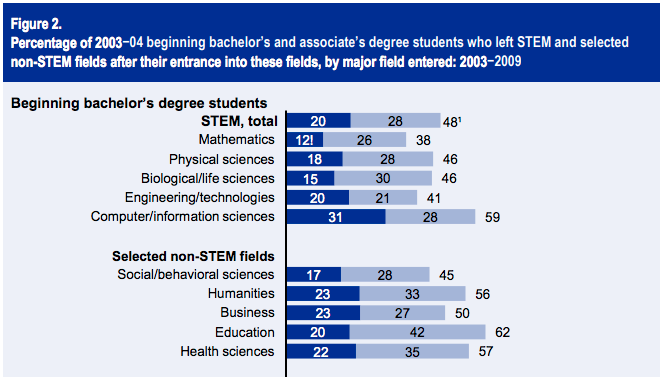
\includegraphics[scale = 0.5]{pic2.png}
\end{frame}

\begin{frame}
  \frametitle{Where do people go?}
  \begin{itemize}
  \item Business is one of the most popular destinations: 22\% of bachelor's degree students who entered STEM fields and later switched majors ended up pursuing business.
  \item The field health sciences was also popular: 20\%.
  \item Education was the least favorite: 6\%.
  \end{itemize}
\end{frame}

\begin{frame}
  \centering
  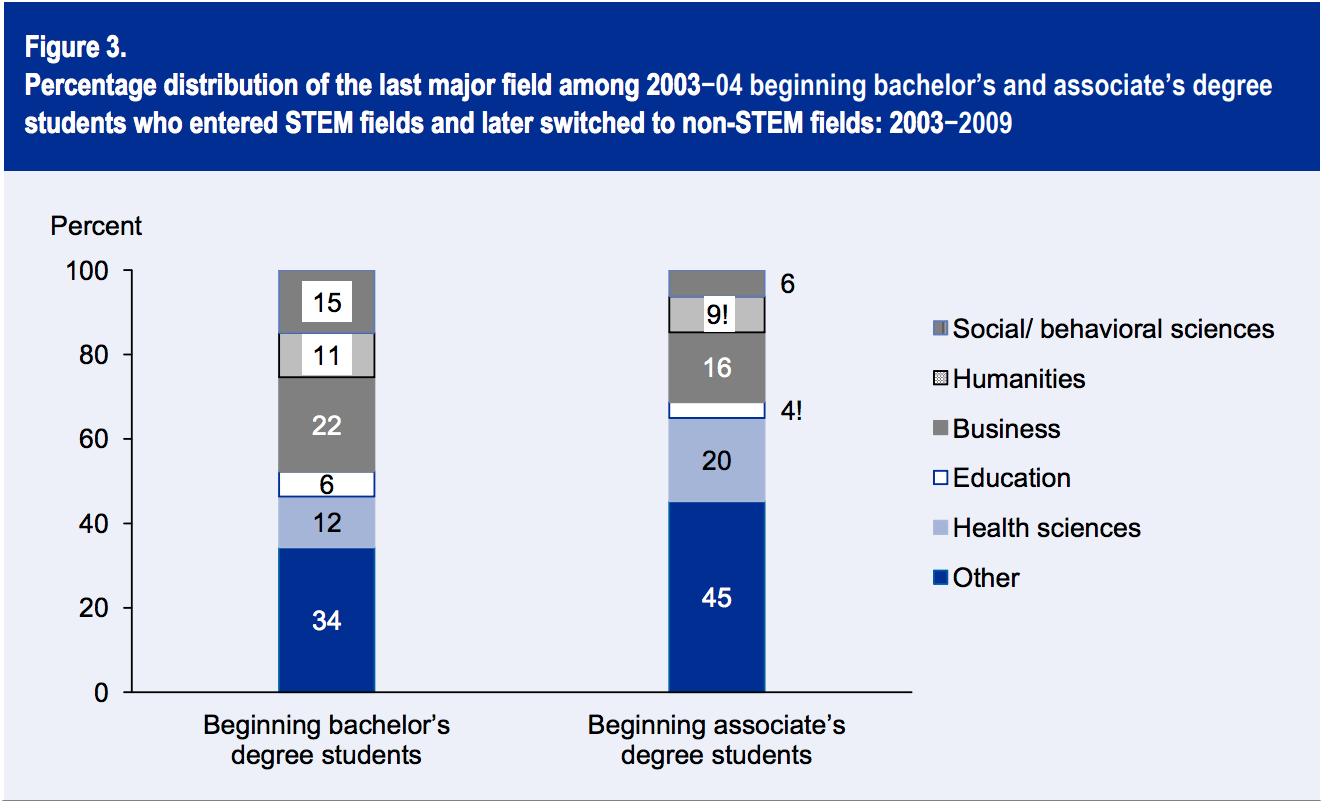
\includegraphics[scale = 0.25]{pic3.png}
\end{frame}

\begin{frame}
  \frametitle{Characteristics of Leavers}
  \begin{block}{Question}
    Why do people leave STEM?
  \end{block}
\end{frame}

\begin{frame}
  \frametitle{STEM coursetaking and performance}
  \begin{itemize}
  \item Students come to college with expectations and preferences based at least in part on
    their high school coursework, achievement, and parental and social influences.
    
  \item These expectations and preferences are reinforced or altered by students’ first-year curricular
experiences, which, in turn, influence their decisions about their subsequent
coursetaking and major field of study (Attewell, Heil, and Reisel 2012; Crisp, Nora,
and Taggart 2009; Huang, Taddese, and Walter 2000; Stinebrickner and
Stinebrickner 2011).
\end{itemize}
\end{frame}

\begin{frame}
  \frametitle{Participation in undergraduate STEM coursework}

  \begin{itemize}
  \item A majority of bachelor’s and associate’s degree students attempted to earn STEM
credits (87 and 78 percent, respectively), and many did so (81 and 67 percent,
respectively) during their first year in college. 

\item On average, STEM credits accounted for 27 percent of all credits earned by bachelor’s and associate’s degree
students in their first year. 
  \end{itemize}
\end{frame}

\begin{frame}
  \frametitle{STEM leavers vs. persisters}
  \begin{itemize}
  \item Despite this widespread participation, however, there were some measurable
differences between STEM leavers and persisters in the number of STEM credits
earned in the first year. 
  \end{itemize}
\end{frame}

\begin{frame}
  \frametitle{Highest level of math course}
  \begin{itemize}
  \item Mathematics is a foundation for all STEM disciplines, and thus, deciding whether to
take mathematics in the first year and what type of math courses to take is crucial to
students’ progression along the STEM pipeline (Shaw and Barbuti 2010).
\end{itemize}
\end{frame}

\begin{frame}
  \frametitle{Highest level of math course}
  \begin{itemize}
\item During their first year in college, 40 percent of bachelor’s degree students did not take
mathematics; 9 percent took only precollege-level math courses; 30 percent took
introductory college-level but no higher-level mathematics; and 21 percent took
calculus or other advanced mathematics (figure 4).
\end{itemize}
\end{frame}

\begin{frame}
  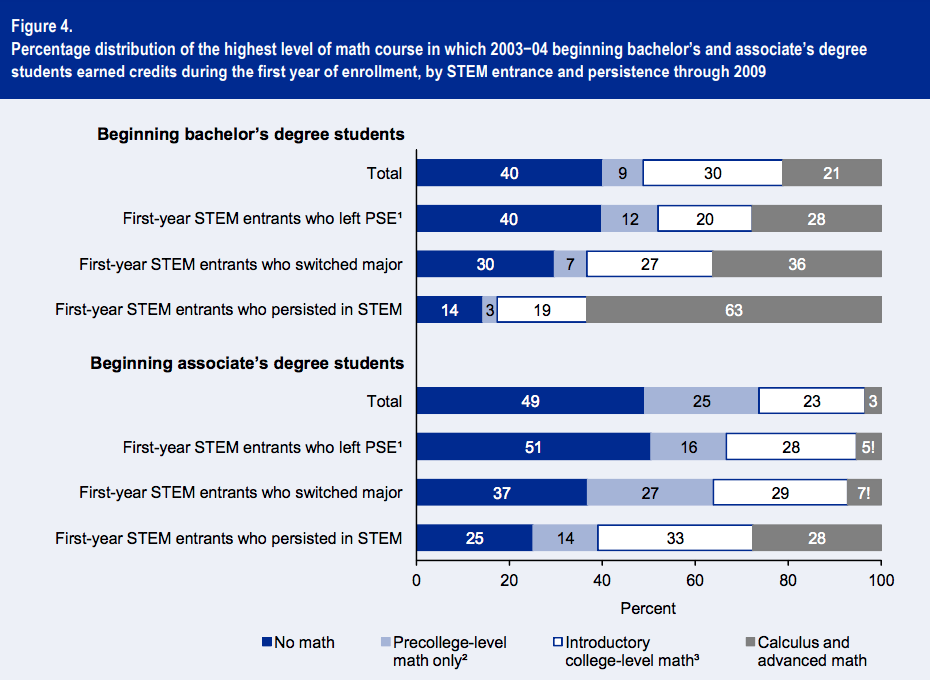
\includegraphics[scale = 0.33]{fig4.png}
\end{frame}

\begin{frame}
  \frametitle{Highest level of math course}
  \begin{itemize}
    \item The level of first-year math coursetaking distinguished STEM leavers from STEM
persisters. 
\item At both the bachelor’s and associate’s degree levels, proportionally more
STEM leavers than STEM persisters did not earn any math credits in their first year,
whereas proportionally more STEM persisters than STEM leavers earned credit in
calculus or advanced mathematics.
\end{itemize}
\end{frame}

\begin{frame}
  \frametitle{Conclusion}
  \begin{itemize}
  \item This is where you come in!
  \item You're teaching their first math class which plays a nontrivial role in their success as a STEM student!
  \end{itemize}
\end{frame}

\begin{frame}
  \frametitle{Conclusion}
  \begin{itemize}
  \item You have an opportunity to make a real impact on students' lives.  Do not take this lightly.
  \item How well you teach MATH 1113 is important to the department (and to everyone else at large).
  \item Even the small things matter.  
  \end{itemize}
\end{frame}


\end{document}
%%% Local Variables:
%%% mode: latex
%%% TeX-master: t
%%% End:
